% NeurIPS-like layout (the official style file is not redistributed here): 5.5in x 9in text, Times, single column.
\documentclass[10pt,letterpaper]{article}
\usepackage[textwidth=5.5in,textheight=9in,top=1in,headheight=12pt,headsep=25pt,footskip=30pt]{geometry}
\usepackage{fontspec}
\setmainfont{texgyretermes}[Extension=.otf,UprightFont=*-regular,BoldFont=*-bold,ItalicFont=*-italic,BoldItalicFont=*-bolditalic]
\setmonofont{texgyrecursor}[Extension=.otf,UprightFont=*-regular,BoldFont=*-bold,ItalicFont=*-italic,BoldItalicFont=*-bolditalic]
\usepackage{amsmath,amssymb,booktabs,graphicx,xcolor,float,caption}
\usepackage[hidelinks]{hyperref}
\usepackage[numbers,sort&compress]{natbib}
\usepackage{titlesec}
\titleformat{\section}{\normalfont\large\bfseries}{\thesection}{0.6em}{}
\titleformat{\subsection}{\normalfont\normalsize\bfseries}{\thesubsection}{0.6em}{}
\titlespacing*{\section}{0pt}{1.0ex}{0.6ex}
\titlespacing*{\subsection}{0pt}{0.8ex}{0.4ex}
\setlength{\emergencystretch}{2em}
\setlength{\parindent}{0pt}
\setlength{\parskip}{5.5pt}
\captionsetup{font=small,labelfont=bf,skip=3pt}
\graphicspath{{../../solutions/mit6.5940/project-mcu-e2e/artifacts/figures/}{../../solutions/mit6.5940/lab3-nas/artifacts/figures/}}

\begin{document}
\begin{center}
\rule{\textwidth}{4pt}\\[0.6em]
{\LARGE\bfseries From a Searched Subnet to an int8 Microcontroller Budget:\\[0.2em]
Visual Wake Words in the Four MLPerf Tiny Columns}\\[0.5em]
\rule{\textwidth}{1pt}\\[1.0em]
{\bfseries ShaneLiu04}\\
MIT 6.5940 (Fall 2024) final project, independent re-implementation\\
\texttt{solutions/mit6.5940/project-mcu-e2e}, \texttt{solutions/mit6.5940/lab3-nas}
\end{center}
\vspace{0.4em}

\begin{center}\begin{minipage}{0.88\textwidth}
\small\textbf{Abstract.}
We take two Visual Wake Words (VWW)~\cite{vww} subnets found by predictor-guided evolutionary search in the OFA-MCUNet~\cite{ofa} design space of Lab~3, and the three VWW models released with MCUNet~\cite{mcunet}, through one pipeline: BatchNorm folding, ONNX export, static int8 post-training quantization, and costing in the four MLPerf Tiny~\cite{mlperftiny} columns (accuracy, latency, flash, peak SRAM).
On the same 4,030 validation images, our 60M-MAC subnet reaches 92.53\% int8 top-1 against 91.37\% for \texttt{mcunet-vww2} at 5\% fewer convolution MACs and an estimated 223~ms versus 234~ms on an STM32F746, paying 190~KB more flash and 88~KB more activation memory; patch-based inference~\cite{mcunetv2} halves that memory for 18\% more MACs.
Three findings matter beyond the numbers: the course MAC counter charges BatchNorm 4~ops per element and inflates MACs by 9--15\%; ONNX Runtime's default entropy calibration is byte-for-byte MinMax; and on a 4,030-image validation set the 92.5\% target of the lab is inside one standard error (0.41 points), so the choice of selection rule decides whether it is met.
Latency on the MCU is \emph{estimated} from TinyEngine's published numbers, not measured.
\end{minipage}\end{center}

\section{Setup}
\textbf{Design space and search (Lab 3).} The supernet is the course OFA-MCUNet (\texttt{mcunet384}): resolution $\{96,\dots,160\}$, width $\{0.5,0.75,1.0\}$, per-block kernel $\{3,5,7\}$ and expansion $\{3,4,6\}$ over 20 elastic blocks, extra depth $\{0,1,2\}$ in 6 stages.
A closed-form efficiency model lists every layer's input/output elements and MACs; on 1,004 subnets it matches the course hook-based counters exactly for MACs, peak activation and parameters, at 0.21~ms instead of 66~ms per subnet.
The accuracy predictor is the course MLP (3$\times$400, L1) on 40k of the 50k measured subnets (validation MAE 0.18 points, Kendall $\tau=0.925$).
Evolution (population 100, 60 generations) is run 20 times per constraint; the 10 best distinct members of each final population, plus the top of an evolution scored by measured holdout accuracy, are all measured (210 per constraint).
The answer is the subnet the predictor ranks first, as the course procedure prescribes; other selection rules are reported in \S\ref{sec:select}.

\textbf{Evaluation.} VWW images from the course package are resized to $r\times r$ and normalized with mean and std 0.5; even indices (4,030) are the validation set, odd indices (4,029) the holdout on which subnet BatchNorm statistics are re-estimated and quantization is calibrated (first 512 images). Validation images are never used for selection.

\textbf{Deployment path.} BN is folded into the preceding conv (max logit change $1.6\times10^{-5}$). Static QDQ quantization in ONNX Runtime 1.31: int8 per-channel weights, uint8 activations, MinMax ranges. The released MCUNet \texttt{.tflite} files are also evaluated with LiteRT, feeding \texttt{pixel}$-128$ as in the release's evaluation script.

\textbf{Costs.} \emph{Flash}: int8 weights + int32 biases + one fp32 scale per output channel. \emph{SRAM}: tensor lifetimes traced with \texttt{torch.fx}, greedy-by-size placement (equal to the liveness lower bound on all five models) and TinyEngine's in-place depthwise~\cite{mcunet}; the patch column takes the cut and split with the smallest peak among those costing $\le 1.3\times$ MACs. \emph{Latency}: a line through TinyEngine's three published VWW points on an STM32F746 (6.0M$\to$27~ms, 11.6M$\to$51~ms, 55.8M$\to$234~ms), $4.15$~ms/M\,MACs $+\,2.45$~ms, maximum residual 1.3\%. Our hook count of the released models' convolution MACs (5.96/11.58/55.77M) agrees with the published 6.0/11.6/55.8M, so the axis of the fit is the right one. x86 latency is batch 1, one thread pinned to one core of a Xeon Platinum 8470Q, median of 300 runs.

\section{Results}
\begin{table}[H]
\centering\small
\caption{The four columns. Accuracy is top-1 on 4,030 VWW validation images. MCU latency is \emph{estimated}. SRAM is the int8 activation arena with in-place depthwise; ``patch'' in brackets is the MAC overhead.}\label{tab:main}
\setlength{\tabcolsep}{3.6pt}
\begin{tabular}{lrrrrrrrrr}
\toprule
model & $r$ & MACs & fp32 & int8 & .tflite & flash & SRAM & SRAM, patch & MCU ms \\
\midrule
\texttt{mcunet-vww0} & 64 & 5.96M & 87.30 & 87.15 & 87.22 & 390K & 56K & 30K (1.24) & 27 \\
\texttt{mcunet-vww1} & 80 & 11.58M & 89.03 & 88.83 & 88.86 & 459K & 88K & 38K (1.16) & 51 \\
\texttt{mcunet-vww2} & 144 & 55.77M & 91.49 & 91.37 & 91.29 & 678K & 162K & 162K (1.01) & 234 \\
ours, 200KB/30M & 128 & 26.05M & 90.37 & \textbf{90.22} & -- & 573K & 160K & 112K (1.09) & 111 \\
ours, 250KB/60M & 160 & 53.14M & 92.56 & \textbf{92.53} & -- & 868K & 250K & 122K (1.18) & 223 \\
\bottomrule
\end{tabular}
\end{table}

\begin{figure}[H]
\centering
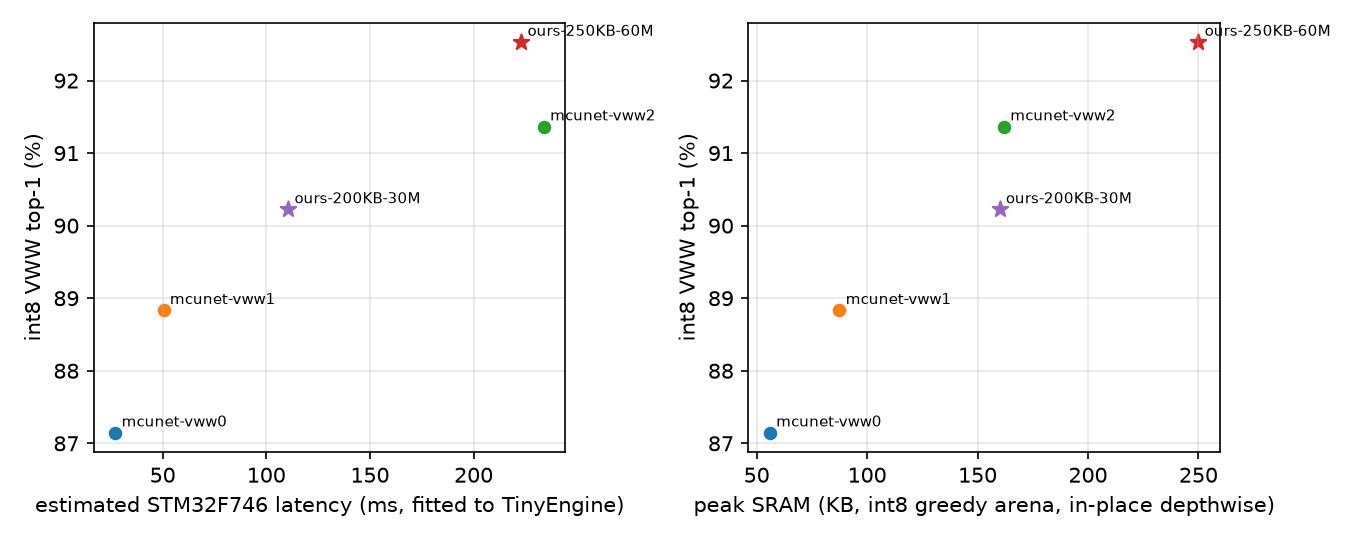
\includegraphics[width=\linewidth]{final_tradeoff.png}
\caption{int8 accuracy against estimated MCU latency (left) and peak SRAM (right). Stars are our subnets.}\label{fig:trade}
\end{figure}

At matched estimated latency our 60M subnet is 1.2 points more accurate than \texttt{mcunet-vww2}; it buys this with resolution 160 and more parameters (flash 868~KB, still inside the F746's 1~MB) and a larger whole-image peak (250 vs.\ 162~KB, both inside 320~KB).
The 30M subnet sits between \texttt{vww1} and \texttt{vww2} on both axes.
int8 costs 0.03--0.20 points on every model, and our ONNX Runtime path is within 0.08 points of the released \texttt{.tflite} files, so the comparison is not an artifact of a weaker quantizer for the baselines.

\textbf{Quantization recipes} (Table~\ref{tab:quant}). Per-tensor weights lose 0.6--2.6 points against fp32.
ONNX Runtime's \texttt{Entropy} method uses a 128-bin histogram and 128 quantized bins, which leaves one candidate threshold, the full range: on all five models the output file is byte-identical to MinMax.
Passing \texttt{num\_bins=2048}, which \texttt{quantize\_static} does not expose, makes the KL search real, and accuracy falls by 0.7--5.2 points.
This repeats, on different networks and a different calibrator, our Lab~2 result that KL clipping on ReLU6 networks discards the outliers that matter.

\begin{table}[H]
\centering\small
\caption{int8 recipes (top-1, \%). Calibration on 512 holdout images; deployed recipe in bold.}\label{tab:quant}
\begin{tabular}{lrrrrr}
\toprule
recipe & vww0 & vww1 & vww2 & ours 30M & ours 60M \\
\midrule
\textbf{MinMax, per-channel, uint8 act.} & 87.15 & 88.83 & 91.37 & 90.22 & 92.53 \\
MinMax, per-tensor & 86.25 & 87.30 & 88.93 & 89.75 & 91.96 \\
Entropy, ORT default (= MinMax bytes) & 87.15 & 88.83 & 91.37 & 90.22 & 92.53 \\
Entropy, 2048 bins & 86.40 & 84.62 & 86.30 & 85.96 & 87.37 \\
Percentile 99.999 & 87.15 & 88.69 & 91.37 & 90.22 & 92.41 \\
MinMax, symmetric int8 act. & 87.25 & 88.59 & 91.24 & 90.07 & 92.51 \\
\bottomrule
\end{tabular}
\end{table}

\textbf{Patch-based inference} (Fig.~\ref{fig:patch}). For models whose peak lies in the first stages, splitting the first 3--5 modules into $2\times2$ or $3\times3$ tiles trades 8--24\% more MACs for 30--67\% less SRAM.
The all-minimum subnet of the space needs 72~KB whole-image, so Lab~3 calls 64~KB infeasible; with a $3\times3$ split after the fourth module its peak is 23.7~KB at $1.21\times$ MACs.
\texttt{mcunet-vww2} is the exception: after in-place depthwise its peak sits late in the network, and no split within $1.3\times$ MACs reduces it (121.5~KB needs $1.33\times$).
Peak SRAM is therefore a property of \emph{where} the largest tensor pair is, which the lab's per-layer rule reports (it agrees with the greedy arena on all five models) but which a single number hides.

\begin{figure}[H]
\centering
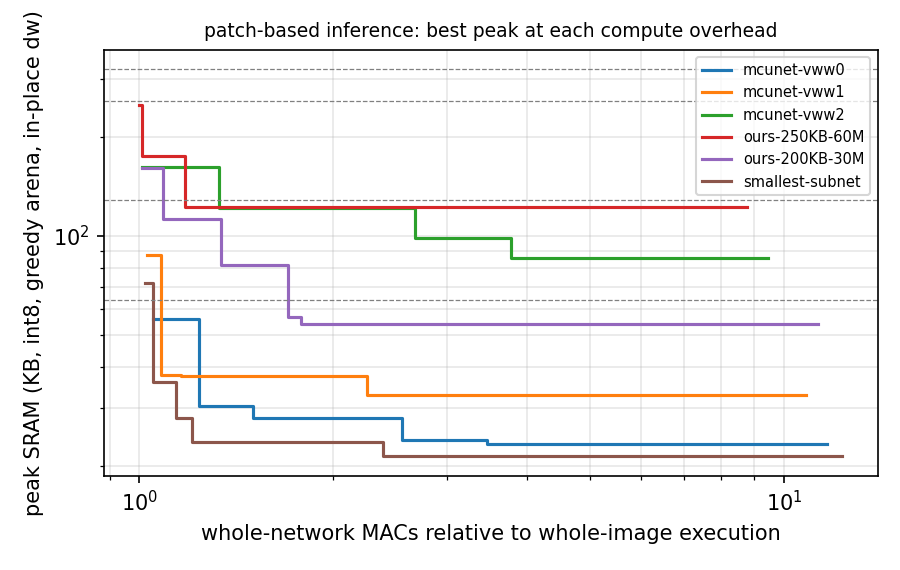
\includegraphics[width=0.78\linewidth]{patch_frontier.png}
\caption{Smallest peak SRAM reachable at each whole-network MAC overhead. Dashed lines: 64, 128, 256, 320~KB.}\label{fig:patch}
\end{figure}

\section{What the search can and cannot resolve}\label{sec:select}
\textbf{The MAC budget is looser than it reads.} The course \texttt{count\_net\_flops} disables BatchNorm's forward but thop still charges each BN 4~ops per output element, so a ``60M'' subnet runs 53.1M convolution MACs; the smallest subnet is 8.30M by the counter and 7.24M by convolutions. Constraints in this report are enforced in the counter's units (as the lab grades them); latency estimates use convolution MACs.

\textbf{Selection noise.} With 4,030 validation images, the standard error of a 92.5\% accuracy is 0.41 points. Among the 210 measured candidates for 250KB/60M, holdout and validation accuracy agree barely at all (Kendall $\tau=0.05$); 67 candidates reach 92.5\% on validation.
The predictor's top pick reaches 92.556\% (holdout 92.60); the holdout's top pick reaches 92.333\% (holdout 92.83), a winner's curse; the best validation accuracy among the candidates is 92.829\% but cannot be selected without using the test set.
For 200KB/30M the corresponding numbers are 90.372, 90.422 and 90.868\% (bar 90\%). A plain 5-seed search picked by holdout gives 92.481\% and 90.447\%.
We report the predictor's pick, decided before looking at validation accuracy, and read ``92.556 $\ge$ 92.5'' as ``indistinguishable from the bar, reached by the stated procedure''.

\begin{figure}[H]
\centering
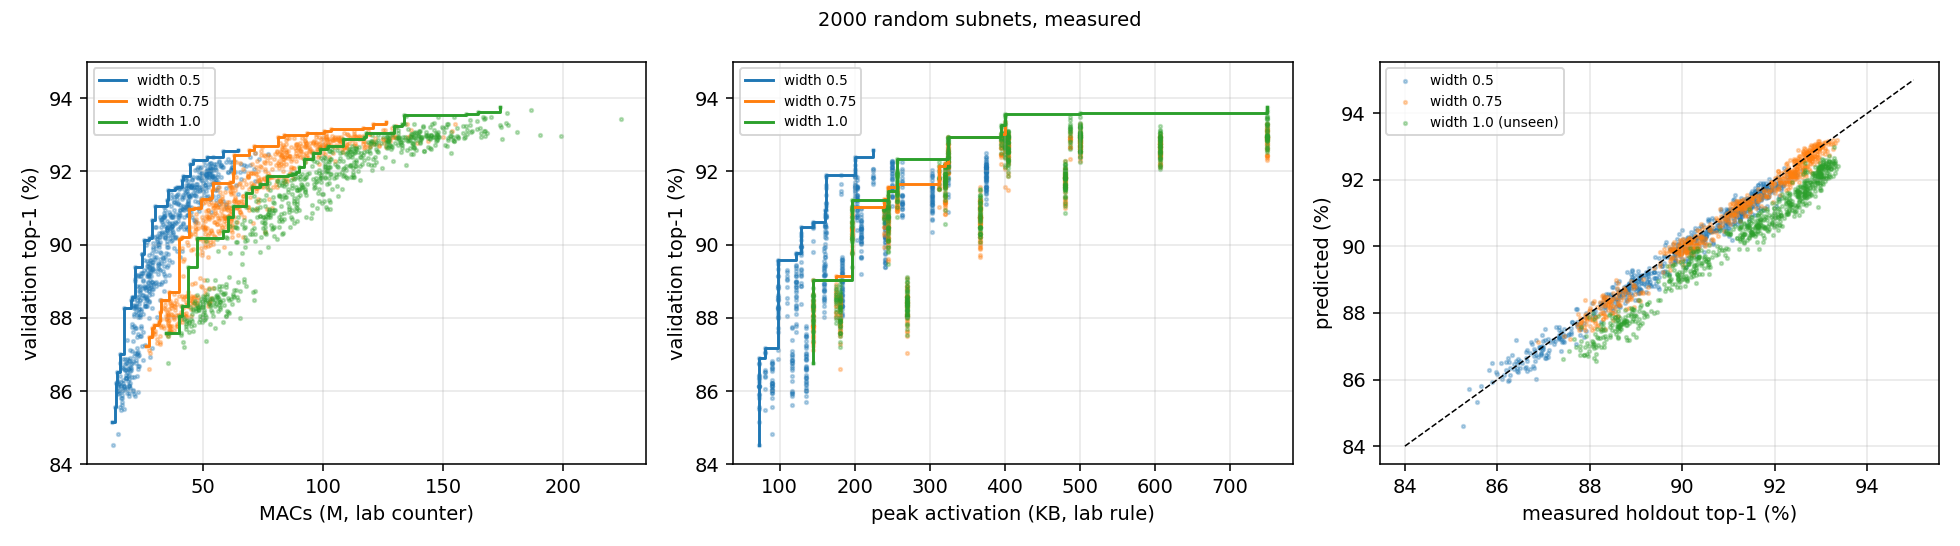
\includegraphics[width=\linewidth]{pareto.png}
\caption{2,000 random subnets, measured. Left/centre: validation accuracy against counter MACs and peak activation with per-width fronts. Right: predictor against measured holdout accuracy; width 1.0 never appears in the predictor's training data.}\label{fig:pareto}
\end{figure}

\textbf{Out-of-distribution widths.} The course sampler draws width from \texttt{range(len(widths)-1)}, so the 50k accuracy dataset has no width-1.0 subnet. On 2,000 freshly measured subnets the predictor's holdout MAE is 0.20--0.21 points for widths 0.5/0.75 but 0.93 for width 1.0, almost all of it bias ($-0.93$), with ranking intact ($\tau=0.88$); it will steer a search away from width 1.0 for reasons that are not accuracy. At equal MACs the width-0.5 front is the highest anyway (Fig.~\ref{fig:pareto}), and the best of the 2,000 random subnets under 256KB/60M is 92.41\%, below the searched 92.56\%.

\section{Limitations}
No board was used: MCU latency assumes TinyEngine's throughput on our layer shapes equals that on MCUNet's (SE blocks and $7\times7$ depthwise kernels differ), and SRAM is a planner's arena, not TinyEngine's generated code; neither includes I/O buffers, stack or kernel workspace. Our subnets had BN re-estimated on the holdout half of the same image pool; whether the released models' training data overlaps this validation set was not checked. Differences below about 0.4 points are not significant at this test-set size.

\begin{thebibliography}{9}\small
\bibitem{mcunet} J.~Lin, W.-M.~Chen, Y.~Lin, J.~Cohn, C.~Gan, S.~Han. MCUNet: Tiny Deep Learning on IoT Devices. \emph{NeurIPS}, 2020.
\bibitem{mcunetv2} J.~Lin, W.-M.~Chen, H.~Cai, C.~Gan, S.~Han. MCUNetV2: Memory-Efficient Patch-based Inference for Tiny Deep Learning. \emph{NeurIPS}, 2021.
\bibitem{mlperftiny} C.~Banbury, V.~J.~Reddi, P.~Torelli, et~al. MLPerf Tiny Benchmark. \emph{NeurIPS Datasets and Benchmarks}, 2021.
\bibitem{ofa} H.~Cai, C.~Gan, T.~Wang, Z.~Zhang, S.~Han. Once-for-All: Train One Network and Specialize it for Efficient Deployment. \emph{ICLR}, 2020.
\bibitem{vww} A.~Chowdhery, P.~Warden, J.~Shlens, A.~Howard, R.~Rhodes. Visual Wake Words Dataset. arXiv:1906.05721, 2019.
\end{thebibliography}
\end{document}
